%% This file is part of the Annie's Lasso project.
%% Copyright 2015 the authors.  All rights reserved.

% To-Do
% -----
% - make full outline
% - get to zeroth draft
% - audit for usage of vector and list
% - search for all occurrences of DWH, AC, or MKN in the text and fix them.

% Style Notes
% -----------
% - Use \acronym{NASA} for acronyms like NASA.
% - The label list \ell is a *list*; the vectorization v(ell) is a *vector*.

\documentclass[12pt,preprint]{aastex}
\usepackage{amsmath,amssymb}

\newcommand{\project}[1]{\textsl{#1}}
\newcommand{\TheCannon}{\project{The~Cannon}}
\newcommand{\acronym}[1]{{\small{#1}}}
\newcommand{\sdss}{\project{\acronym{SDSS-IV}}}
\newcommand{\apogee}{\project{\acronym{APOGEE2}}}
\newcommand{\aspcap}{\project{\acronym{ASPCAP}}}
\newcommand{\dr}{\acronym{DR12}}
\newcommand{\logg}{\log g}
\newcommand{\mh}{\mathrm{[M/H]}}
\newcommand{\Teff}{T_{\mathrm{eff}}}
\newcommand{\Dvector}[1]{\boldsymbol{#1}}
\newcommand{\vectheta}{\Dvector{\theta}}
\newcommand{\vecv}{\Dvector{v}}
\newcommand{\argmin}[1]{\underset{#1}{\operatorname{argmin}}\,}

\begin{document}

\title{\textsl{The Cannon 2:} A data-driven model of stellar spectra \\
       for detailed chemical abundance analyses}
\author{AC, DWH, MKN, others}

\begin{abstract}
% context
In previous work, we have shown that it is possible to train a generative
probabilistic model for stellar spectra using a training set of stars, each labeled with known
physical attributes ($\Teff$, $\logg$, $\mh$), and then use that model to infer labels for
unlabeled stars, even stars with lower signal-to-noise observations.
% aims
Here we ask whether this is possible when the dimensionality of the chemical
abundance space is large
(15 abundances: C, N, O, Na, Mg, Al, Si, S, K, Ca, Ti, V, Mn, Fe, Ni)
and the model is non-linear in its response to abundance and parameter changes.
% methods
We adopt ideas from compressed sensing to limit overall model complexity (number
of non-zero model parameters) while retaining model freedom.
The training set is a set of YYY red-giant stars with high signal-to-noise
spectroscopic observations and stellar parameters and abundances taken from the
\apogee\ Survey.
% results
We find that we can successfully train and use a model with 17 stellar labels.
Cross-validation shows that the model does a good job of inferring all 17 labels
(with the exception of XXX), even when we degrade the signal-to-noise of the
validation set by discarding some of the spectroscopic observing time.
The model dependencies make sense; the derivatives of the spectral mean model
with respect to abundances correlate well with known atomic lines.
We deliver open-source code and also stellar parameters and 15 abundances for a
set of ZZZ stars.
\end{abstract}

\section{Introduction}


The detailed surface abundances of a star reflect its formation environment
and the supernova(e) that preceded it.  Minute perturbations in the properties
of either can produce subtly different chemical abundance patterns on successive
generations of stars.  This chemical abundance signature largely remains 
constant in the stellar photosphere throughout a star's lifetime, thereby 
providing a fossilised record of the gas composition during formation and the 
imprinted signature of stars that preceded it.  The variation between these
signatures is small, implying that it is difficult to distinguish subtle 
chemical patterns from different formation sites.  However if they were 
distinguishable, a sufficiently large collection of stellar abundances would 
unambiguously unravel the complete chemical evolution of the Milky Way.


There are some exceptions to this line of reasoning: the abundances of some
elements can (and do) change throughout a star's lifetime.  However these are
subtle signatures that are reflective of intriguing astrophysical phenomena:
atomic diffusion, evolutionary mixing, the presence (or accretion) of 
exoplanets, material transfer from a stellar binary companion, and countless
other scenarios.  In the same way that precise abundances are required to 
identify unique chemical formation signatures, precise abundances are necessary
to distinguish minute evolutionary or environment differences between subsets of
stars.  In these scenarios we argue most astrophysicists care less about
accuracy; it is the abundance precision that imparts discovery and understanding
of these astrophysical phenomena.  Indeed, in most studies of stellar
astrophysics \textit{an increase in precision yields far more astrophysical 
insight than a comparable increase in accuracy}.


For these reasons a comprehensive catalog of \textit{precise} detailed chemical
abundances would revolutionise our understanding of planetary, stellar, and 
galactic astrophysics.  This goal has only recently become feasible given the 
increasing volume and quality of stellar spectra obtained in the last decade.  
Specifically, large surveys are obtaining high-resolution 
($\mathcal{R} \gtrsim 20,000$), high signal-to-noise (S/N) ratio spectra for
$\sim10^{5}$---$10^{6}$ stars across all components of the Galaxy.  This is a
sharp relative increase in data volume, which has mandated the automatic
analysis of stellar spectra, and persuaded dozens of groups to produce bespoke
pipelines.



Most automated pipelines have grown from classical, manual methods.  That is to
say, there has been relatively little work on unconventional methods to analyse
spectra.  Spectroscopists have hard-coded their intuition (or subjectivity),
with arbitrary heuristics to decide issues of wavelength masks, convergence
criteria, etc.  Most of these decisions are based on optimizing the resultant
accuracy for a few stars with extremely high quality data (e.g., high S/N).  As
a result, these heuristics are frequently incomparable for more data with more
modest (and representative) S/N ratios.  Therefore, for most stars in the sample,
it can be trivially shown from repeat or blind experiments that that individual
pipelines yield demonstrably imprecise abundances for S/N ratios that are 
most typical in the data.  Moreover, results from individual pipelines vary 
significantly with respect to each other, with abundance differences an order
of magnitude larger than the aforementioned astrophysical signatures.
%Thus, while there has been substantial effort in automating classical analysis
%techniques, they are generally imprecise at modest S/N ratios, and yield
%different and inaccurate results when compared against each other.

Considerable efforts have also focussed on improving the accuracy of physical
models.  Indeed it is impossible to measure physical properties of stars (or 
their chemical abundances) accurately without accurate physical models of 
stellar spectra.  However, physics-based models of stars have a number of known
problems.  The atmospheres are generally one-dimensional; three-dimensional
models remain computationally impractical for more than just a few stars.  As a
consequence of the limited atmosphere dimensionality, crude (knowningly 
incorrect) approximations for the convection and turbulence become necessary. 
Although grids of three-dimensional hydrodynamic models have been produced 
and averaged to one-dimensional approximations, these models still assume local
thermodynamic equalibrium (LTE).  Properly accounting (or even approximating) 
departures from LTE is a formidable analytic and computational challenge.
Lastly, while laboratory efforts have thoroughly improved much of the faulty
atomic and molecular data, this process is unquestionably incomplete.  For these
reasons there are some spectral features that are much better understood than
others.  As a consequence, physics-based methods are restricted to spectral
regions or parameter space that are understood marginally better, which vastly
limits their applicability and interpretability by construction.


%Even the opacities employed by modern radiative transfer codes are polynomial approximations that are decades old.

In detail, physics-based models do not explain all pixels of stellar 
spectroscopy at the precision with which we are currently observing.  The data
quality have outgrown the classical methods used to analyse them.  This led us 
to build \TheCannon\footnote{It is important (to us) to note that \TheCannon\ 
is named not after a weapon but instead after Annie Jump Cannon, who was the 
first to correctly order stellar spectra in temperature order (and who did so
by looking at the data, and without any use of physics-based models).} 
(\citealt{tc}), a data-driven---as opposed to physics-based---model for stellar
spectra.  \TheCannon\ is a data-driven model, but it differs from standard 
machine-learning approaches because it contains an explicit noise model. Given a
representative set of stars with known labels of high-fidelity (see below), 
\TheCannon\ is a generative model for stellar spectra based on a linear 
combination of the labels.



%DWH: Summarize what it does and what it can be used for.
%DWH: Mention some users and projects, past, current, and future.
%DWH: Cite some relevant literature.


Before we introduce the construction of the model and the tests we employed to
evaluate it, we first need to introduce the relevant terminology.  In all that 
follows, we will call stellar parameters ($\Teff$ and $\logg$) and the full set
of 15 chemical abundances collectively ``labels''.  This unifies and collapses 
the phrase ``stellar parameters and chemical abundances'' to a word, and 
connects to relevant terminology for supervised methods in the machine-learning
and statistics literatures.  Consider a spectroscopic survey that contains 
\emph{survey objects}.  Within that set of survey objects is a subset of stars 
where the data have high signal-to-noise ratios such that we can assert the 
labels are reported with high fidelity.  We will call this sample the 
\emph{labelled set}, whereas all other survey objects are categorized to the
\emph{unlabelled set}.  That is to say, although objects in the 
\emph{unlabelled set} may have reported labels, we are going to construct
(train) \TheCannon\ using data in the labelled set and estimate (test) labels 
for those in the unlabelled set.  This means that \TheCannon\ can transfer 
labels from high signal-to-noise training-set stars to low signal-to-noise 
test-set stars; that is, the training set and the test set do not need to be 
statistically identical.  This is related to the fact that \TheCannon\ is an 
interpretable model; the internals of the model are the dependencies of the 
spectral expectation and variance on wavelength and physical parameters of the 
star.


%DWH: Define the words ``train'', ``validate'', and ``test''.  And maybe ``predict'' too?

%DWH: Labels for data at wavelengths where there are no good labels.

%DWH: Labels that are consistent across surveys and wavelengths.


%DWH: Should we be saying things about the fact that the model is probabilistic?
%It takes as input stellar labels and gives as output a pdf for stellar spectra?

%DWH: 

In the first work we did with \TheCannon, we only used a small number of labels
(three in the original work, and four or five in late work; \citealt{tc, age}). 
Here we were guided by thoughts related to density estimation: As the length of 
the label list $K$ grows, so too does the model complexity.  Sampling well a 
$K$-dimensional label space takes a training set the size of which scales 
exponentially (or worse) with $K$.  Subsequent experiments, however, did not 
bear this out. We found that we can transfer many labels from the training set 
to the test set, with training sets of thousands of stars.  The fundamental 
reason is that \TheCannon\ is \emph{not} a density estimator!  It is more like 
an \emph{interpolator}, which effectively finds stars in the training set that 
are close to the test star, and transfers labels, using the smooth polynomial 
model as a kind of regularizer.


The capacity to extend to a larger set of $K$ labels without significant
computational detriment offers tantalizing opportunities.  The most 
straightforward would be to include abundances of individual elements as labels.
However in doing so, it can be shown that a standard \emph{Cannon} model yields
$\theta$ derivatives (see next section) that are incompatible with expectations
from physics: there may be an abundance label with non-zero contributions at all
pixels, but physically we know that spectral lines of a single element do not 
contribute across all wavelengths.  

For this reason alone we know the problem is sparse.  Here we exploit this 
information to the fullest, using standard regularization methods to discover
and enforce sparsity. We consider the \emph{entire} 17-dimensional label space 
produced by the \apogee\ \aspcap\ pipeline.  We accept the \aspcap\ labels for 
the highest signal-to-noise stars, and adopt these stars and their labels as the
training set.  We show by validation that we can transfer these labels to much 
lower signal-to-noise stars, with reduced precision but no strong biases.  We
then use the system to label all of the stars in the \apogee\ \dr\ data set.


%DWH: The differences between measurement and prediction...

%DWH: Etc!

\section{Method}

\noindent{}We assume the following about \TheCannon\ and the \apogee\ \dr:

%The assumptions of \TheCannon\ are the following:
\begin{itemize}
\item
Stars with similar labels (parameters and abundances) have similar spectra.
\item
The expectation of the spectrum of a star is a smooth function of the values of 
the labels for that star.  Further than this, we assume that the function is so 
smooth it is reasonably approximated with a quadratic form in label space.
\item
The resolution of all \apogee\ spectra are identical, all spectra are calibrated
to the same rest wavelength grid, the noise is Gaussian and independent from 
pixel to pixel (with correctly known variances at the pixel level).  
Importantly, we are \emph{not} assuming that different stars have similar noise
variances, nor that the training, test, and prediction sets have the same noise 
model.
\item
We have a training set of stars with accurate labels, where ``accurate'' is 
defined by the accuracy requirements of the output labels.  It might be more 
accurate to say that we are assuming that the training-set stars have 
\emph{consistent} labels (consistent with the assumptions of smoothness, above).
% ARC: I don't think we even care if ASPCAP is accurate or not -- we aren't 
technically assuming accuracy in the training set, are we? We are only assuming 
consistency in all of our criteria for deciding what should or should not be in 
the labelled set (and thus the training set).
\item
The training set is representative, in the sense that the training-set stars 
span the label space similarly to how any test or prediction set spans the label
space.
\item
We assume our continuum normalization procedure (described below) is consistent.
Note that we do not require \emph{true} continuum-normalization in the classical
sense because any offset (even a label-dependent residual due to a strong 
absorption line) can be captured by the model.  Instead we require that our 
normalization procedure is invariant with respect to S/N ratios.
\end{itemize}


\noindent{}Given these assumptions, the model we adopt is
\begin{eqnarray}
  y_{jn} &=& \vecv(\ell_n)\cdot\vectheta_j + e_{jn}
  \label{eq:model}\quad ,
\end{eqnarray}
where $y_{jn}$ is the data for star $n$ at wavelength pixel $j$,
$\vecv(\ell_n)$ is a function that takes as input
the label list $\ell_n$ of length $K$ for star $n$
and outputs a vector of length $D>K$ of functions of those labels,
$\vectheta_j$ is a vector of length $D$ of parameters controlling the model at wavelength pixel $j$,
and $e_{jn}$ is a noise draw or residual.  We refer to $\vecv(\ell_n)$ as ``the vectorizing function'', which allows for arbitrarily complex functions that might not be simple polynomial expansions of the label list $\ell_n$.  
Inasmuch as the model is good, the noise values $e_{jn}$ can be taken to be
drawn from a Gaussian with zero mean and variance $\sigma^2_{jn}+s^2_j$,
where $\sigma^2_{jn}$ is the pipeline-reported uncertainty variance on datum
$y_{jn}$ and $s^2_j$ is a parameter describing excess variance at wavelength pixel $j$.

Two comments about the model (\ref{eq:model}).
The first is that, because the $e_{jn}$ are thought of as being drawn from a 
probability density function (pdf), it is a probabilistic model for the spectral
data $y_{jn}$.
The second is that the output of the function $\vecv(\ell)$ can be thought
of as a row of the ``design matrix'' that defines the possible freedom
given to the spectrum expectation model.

In the \emph{training step}, we fix the $K$-lists of labels $\ell_n$
for all training-set stars $n$.
We seek, at each wavelength pixel $j$, the $[D+1]$ parameters
$\vectheta_j,s^2_j$ that optimize a penalized likelihood:
\begin{eqnarray}\label{eq:train}
  \vectheta_j,s^2_j &\leftarrow& \argmin{\vectheta,s^2}\left[
    \sum_{n=0}^{N-1} \frac{[y_{jn}-\vecv(\ell_n)\cdot\vectheta]^2}{\sigma^2_{jn}+s^2}
    + \sum_{n=0}^{N-1} \ln(\sigma^2_{jn}+s^2)
    + \Lambda_j\,Q(\vectheta)
    \right]
  \quad ,
\end{eqnarray}
where $\Lambda_j$ is a regularization parameter, and $Q(\vectheta)$ is a 
regularizing function that encourages parameters to take on zero values.
The regularizing function takes a $D$-vector as input and returns a
scalar value.
We call this penalized likelihood---the argument of the
argmin in equation~(\ref{eq:train})---the \emph{training scalar}.
We will adopt for the regularizing function $Q(\vectheta)$ in the training scalar a
modification of L1 regularization, discussed below.
Although the training-step optimization problem will not in general be
convex, we can make choices for $Q(\vectheta)$ (and we will) to make the
problem such that it would be convex at any fixed value of $s^2$; for
this reason it will tend to optimize well in most cases of interest.

The regularization parameter $\Lambda_j$ sets the strength of the
regularization; as $\Lambda_j$ increases, the number of non-zero
components of the parameter vector $\vectheta_j$ will decrease.
We give the regularization parameter a subscript $j$ because in
general we can set it differently at every wavelength.
This makes sense, because different wavelengths have very different
dependences on different components of the label list $\ell$.
In what follows, we will set the value of the $\Lambda_j$ by
validation or cross-validation or possibly based on physical arguments
about what matters!


In the \emph{test step}, we fix the parameters $\vectheta_j,s^2_j$ at all
wavelength pixels $j$.
We seek, for each test-set star $m$, the $K$-list of labels $\ell_m$
that optimizes the likelihood:
\begin{eqnarray}\label{eq:test}
  \ell_m &\leftarrow& \argmin{\ell}\left[
    \sum_{j=0}^{J-1} \frac{[y_{jm}-\vecv(\ell)\cdot\vectheta_j]^2}{\sigma^2_{jm}+s^2_j}
    \right]
  \quad .
\end{eqnarray}
Because the vectorizing function $\vecv(\ell)$ is non-linear, the
test-step optimization is not convex.
However, the fact that there are many pixels $j$ acting, each of which
has a different functional dependence on the labels in the label list
$\ell$, tends to make the optimization (in practice) find a good value
for the label list $\ell$.
We call this partial log likelihood---the argument of the
argmin in equation~(\ref{eq:test})---the \emph{test scalar}.

The model freedom of \TheCannon\ is set by the vectorizing function
$\vecv(\ell)$---which takes the $K$-element label list $\ell$ and expands
it into a $D$-dimensional vector of components for the linear
model---and the regularization $\Lambda_j\,Q(\vectheta)$.
Because we want the (simple, see below) regularization to treat the
different parameters (the different components of $\vectheta$) in some
sense ``equally'', we have to make sensible choices in the vectorizing
function $\vecv(\ell)$.
One thing that the vectorizing function $\vecv(\ell)$ can do is offset the
labels by some kind of fiducial (mean, median, or other central)
value, such that $\vecv(\ell)=0$ is at a central location in the label
space.
Another is to divide out a scale, because, for example, $\Teff$ values
are in the thousands, but $\logg$ values are of order unity.
If scale is not divided out, the (isotropic in $\vectheta$)
regularization will be much more harsh, effectively, on some
parameters than others.

In what follows, we adopt the median value in the training set for
each label value as the fiducial offset for that label.
We choose a dimensionless constant $Q$ times the label range (defined
as the difference between the 97.5th percentile and the 2.5th
percentile of the training set along each label direction) as the
label scale for that label.
DWH: We need an equation array here giving the above...

For the regularizer $Q(\vectheta)$ we adopt a variant of L1
regularization; we set
\begin{eqnarray}
  Q(\vectheta) &=& \sum_{d=1}^{D-1} |\theta_d|
  \quad,
\end{eqnarray}
where the sum is over the $[D-1]$ components of $\vectheta$, excluding
the zeroth component because we don't ever expect that component to
vanish.
(Forgive a notational similarity here: When we subscript $\vectheta$ with
$j$ we mean ``the $D$-vector of parameters associated with wavelength
pixel $j$''; when we subscript $\theta$ with $d$ we mean ``the single
parameter along coordinate axis $d$ in the $D$-dimensional $\vectheta$
vector space.)
There is a great deal of theory about this kind of regularization; it
is called L1 or the lasso (DWH CITE STUFF).
L1 regularization encourages parameters to vanish precisely but
doesn't break convexity for convex problems.

DWH: To set the amplitude $\Lambda_j$ at each wavelength pixel $j$, we
employ a validation of the following form:....

DWH: Scaling argument that, in general, the best value of $\Lambda_j$
should be on the same order as the number of stars in the training
set....

DWH: Note that the vectorizer scales $\Delta$ play into the
regularization, because the bigger the $\Delta$, the more penalized
the cross (quadratic) terms become relative to the linear terms...

\section{Training, validation, and test data}

We employ the \apogee\ Data Release 12 data to demonstrate the effectiveness
of \TheCannon\ and the regularization approach in a high-dimensional label space.
We constructed our labelled set (recall that the training and validation sets are subsets of the labelled set) using sensible criteria for  
stars in version \texttt{v603} from the \aspcap\ 
pipeline, and used fluxes from the individual \texttt{aspcapStar} data files.
The \texttt{aspcapStar} files contain (approximately) continuum-normalized 
spectra, often stacked from multiple visits, and an error array for those 
fluxes.  All spectra have been placed at rest-frame (vacuum wavelengths), and
resampled onto a common log-wavelength scale. In total, there are NNNNN science
objects.

We employed several quality criteria to distill a robust yet representative 
labelled set: We removed any stars with problematic flags from the \aspcap\
pipeline, requiring \texttt{ASPCAPFLAG = 0}.  We excluded stars with 
signal-to-noise ratios outside the range of 200-300, and stars with a radial 
velocity scatter larger than 1~km~s$^{-1}$.  We further demanded that
our training set include reported abundances in all 15 elements (C, N, O, Na, 
Mg, Al, Si, S, K, Ca, Ti, V, Mn, Fe, and Ni), and restricted the abundance range
such that $2 > \mathrm{[X/Fe]} > -2$, $\mathrm{[Fe/H]} > -3$, and 
$[\alpha/\mathrm{Fe}] > -0.1$.  A visual comparison of the [V/H] labels
with other (Fe-peak) abundance labels showed that many stars in the training set had
spurious measurements of [V/H]. For this reason we further constrained the
labelled set such that $\mathrm{[V/Fe]} > -0.6$.  The distilled sample
includes 14,141 red giant branch stars that will form our labelled set, with [Fe/H] labels ranging from
$\mathrm{[Fe/H]} = [-2.10, 0.30]$. 

DWH: How did we combine the ivars and the flags to make better ivars?

DWH: What is different about our continuum normalization from everyone else's?

DWH: It is \emph{pseudo-continuum normalization}.

DWH: Emphasize that if you use traditional continuum methods,
\TheCannon\ will give \emph{very bad results}.  Don't do that.

DWH: We re-stacked the spectra ourselves, because we are that hardcore.

DWH: Line-spread-function variations exist and we suck in this regard.


%DWH: Define the various possible sets of ``labeled'' stars and the set of ``unlabeled''
%stars, for our various purposes.

%DWH: Any training set must be a subset of the
%labeled stars.
%We are going to use different subsets for different trainings of \TheCannon.

To demonstrate the predictive power and accuracy of the method, we
will (below) perform a conservative cross-validation using cyclic
training, validation, and test subsets of the labeled data:
To each star in the input set of labeled stars (the superset of any
possible training set we might use), we assign an integer $0\leq
q<10$, with uniform probability across all 10 possible values of $q$.
This permits a very conservative 10-fold cross-validation, in which we
choose $8/10$ of the labeled data as the training set, a disjoint
$1/10$ as a validation set for choosing the hyper-parameters
$\Lambda_j$, and a mutually disjoint $1/10$ as a test set for
prediction.
This train--validate--test framework is very conservative, because there
is no way, for each choice of train, validate, and test sets from the
labeled data, for the test set to influence the choice of
hyper-parameters, or indeed for any information to flow from the test
set into the training.

When \TheCannon\ is used to label the full unlabeled set, we train on
the entire unlabled data set (the largest possible training set) and
use values for the hyper-parameters $\Lambda_j$ derived from the
10-fold cross-validation experiment, as we will describe below.

% ARC: Figure: HRD (coloured by [Fe/H]) of the labelled set.

\section{Experiments}

\paragraph{Validation for hyper-parameter selection:}
Hello World!

\paragraph{Three-label case:}
Hello World!

\paragraph{Seventeen-label case:}
Hello World!

\paragraph{Label recovery as a function of signal-to-noise:}
Hello World!

\section{Results}

DWH: Do we need this section?

DWh: What can we say about chemical abundance precision and accuracy?

DWH: What can we say about chemical abundance space?

DWH: What can we say about the promise of chemical tagging?

\section{Discussion}


\TheCannon\ is a prediction system: It is designed to predict the
labels for stars.
It has a fundamental assumption that the training set is statistically
identical to the prediction/test set.
If there are covariances in the label space---that is, if stars in the
training set are high in label $X$ whenever they are also high in
label $Y$---then there will be opportunities for \TheCannon\ to get
information about $Y$ from considering data aspects that depend on
$X$ (which, according to the training set, is reliably connected to $Y$).
For this reason, we expect that, given a finite training set, there
will be situations in which lines from one element are used to predict
the abundance of another.
A good example is shown in \figurename~\ref{fig:whatever}, where we
see WHATEVER.
DWH: Yada Yada...


DWH: No accounting for variable spectroscopic resolution, nor
microturbulence nor rotation.

DWH:  Once again, the differences between measurement and prediction...

DWH:  Why is this going to change the World nonetheless?

DWH: All of the code for this project is available with documentation
at \url{http://thecannon.io/}.

\acknowledgements
DWH: Dan Foreman-Mackey (UW) and Hans-Walter Rix (MPIA) and other people...
grants...
\sdss...

\begin{thebibliography}{dummy}\raggedright
\bibitem[Ness et al.(2015a)]{tc} Ness, M., Hogg, D.~W., 
Rix, H.-W., Ho, A.~Y.~Q., \& Zasowski, G.\ 2015, \apj, 808, 16
\bibitem[Ness et al.(2015b)]{age} Ness, M., Hogg, D.~W., 
Rix, H., et al.\ 2015, arXiv:1511.08204 
\end{thebibliography}

\clearpage

\begin{figure}[p]
\caption{Choose two wavelengths (one continuum and one interesting)
  and plot some scatter plots of flux vs various parameters, and also
  cross-validation results for the
  hyper-parameters.\label{fig:onewavelength}}
\end{figure}

\begin{figure}[p]
\caption{Something about hyper-parameters and scatter as a function of
  wavelength.\label{fig:hyperpars}}
\end{figure}

\begin{figure}[p]
\caption{Something about first derivatives of the spectral expectation
  with respect to labels as a function of
  wavelength.\label{fig:derivatives}}
\end{figure}

\begin{figure}[p]
\caption{Show a few sample spectra and demonstrate that the quality of
  the model prediction is extremely good; better than
  \aspcap.\label{fig:correctness}}
\end{figure}

\begin{figure}[p]
\caption{Something showing that our results on the full unlabeled set
  make sense and seem correct!\label{fig:fulltest}}
\end{figure}

\begin{figure}[p]
\caption{Choose two elements that are interesting, and pull apart the
  differences between what we have and what \aspcap\ has for those
  elements.  We are better!\label{fig:elements}}
\end{figure}

\begin{figure}[p]
\caption{Something about the quality of results in the
  cross-validation as a function of the signal-to-noise of what we
  give in the test subset.\label{fig:snr}}
\end{figure}


\begin{figure}[p]
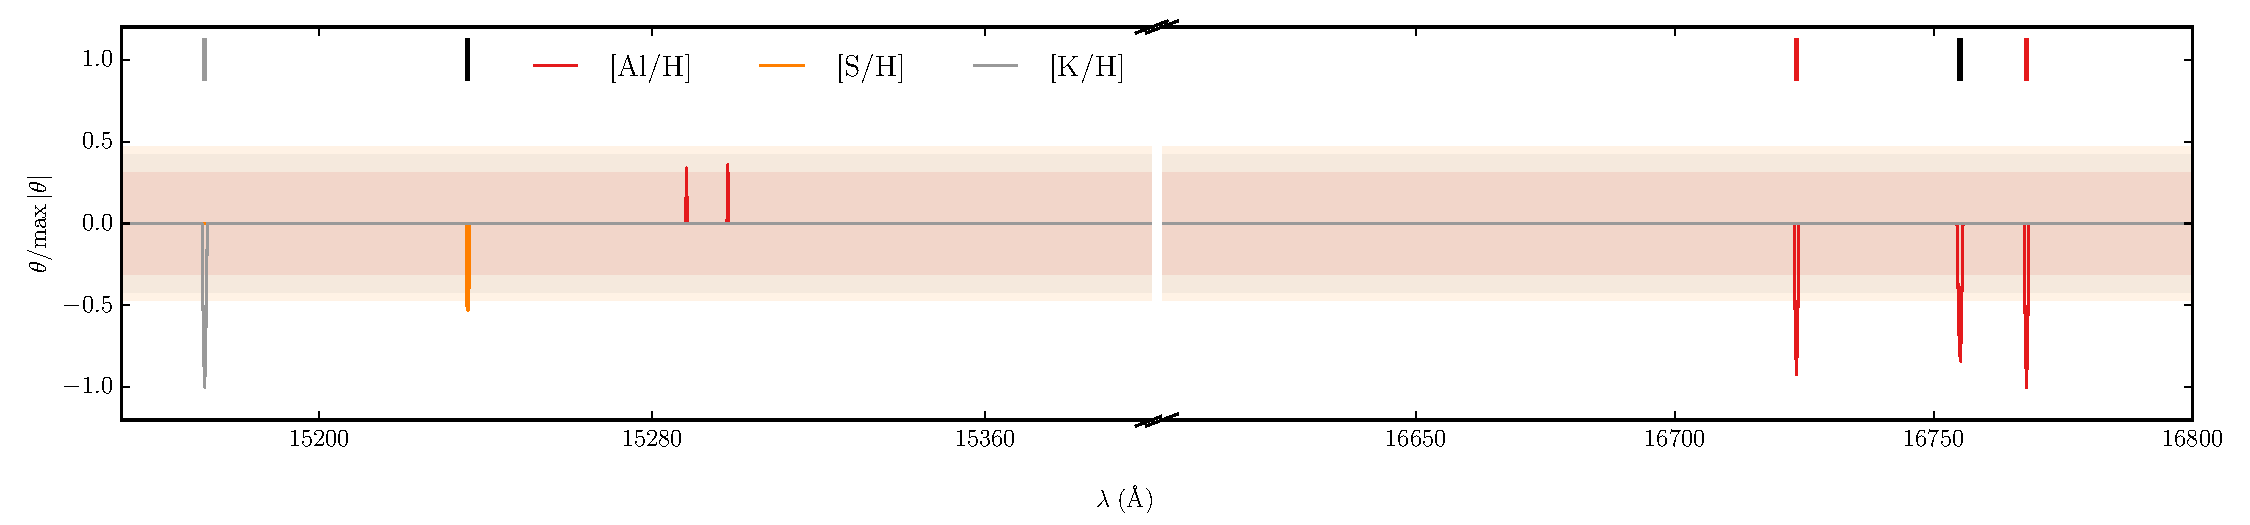
\includegraphics[width=\textwidth]{sparse-first-order-coefficients.pdf}
\caption{Normalized (to the maximum derivative value at any $\theta$) first-order derivatives for [Al/H], [S/H], and [K/H] from a regularized Cannon model with $\Lambda = 10^{3.5}$ and $f = 20$. For the sake of clarity, we have only shown $\theta$ values that exceed the shaded region. The top markings for K and Al correspond to the lines used by Smith et al. The black markers indicate 'Missing' or 'Unknown' lines in the APOGEE spectra according to Shetrone et al. Here we identify these elements from our model derivatives.  \label{fig:inferring-lines}}
\end{figure}

\begin{figure}[p]
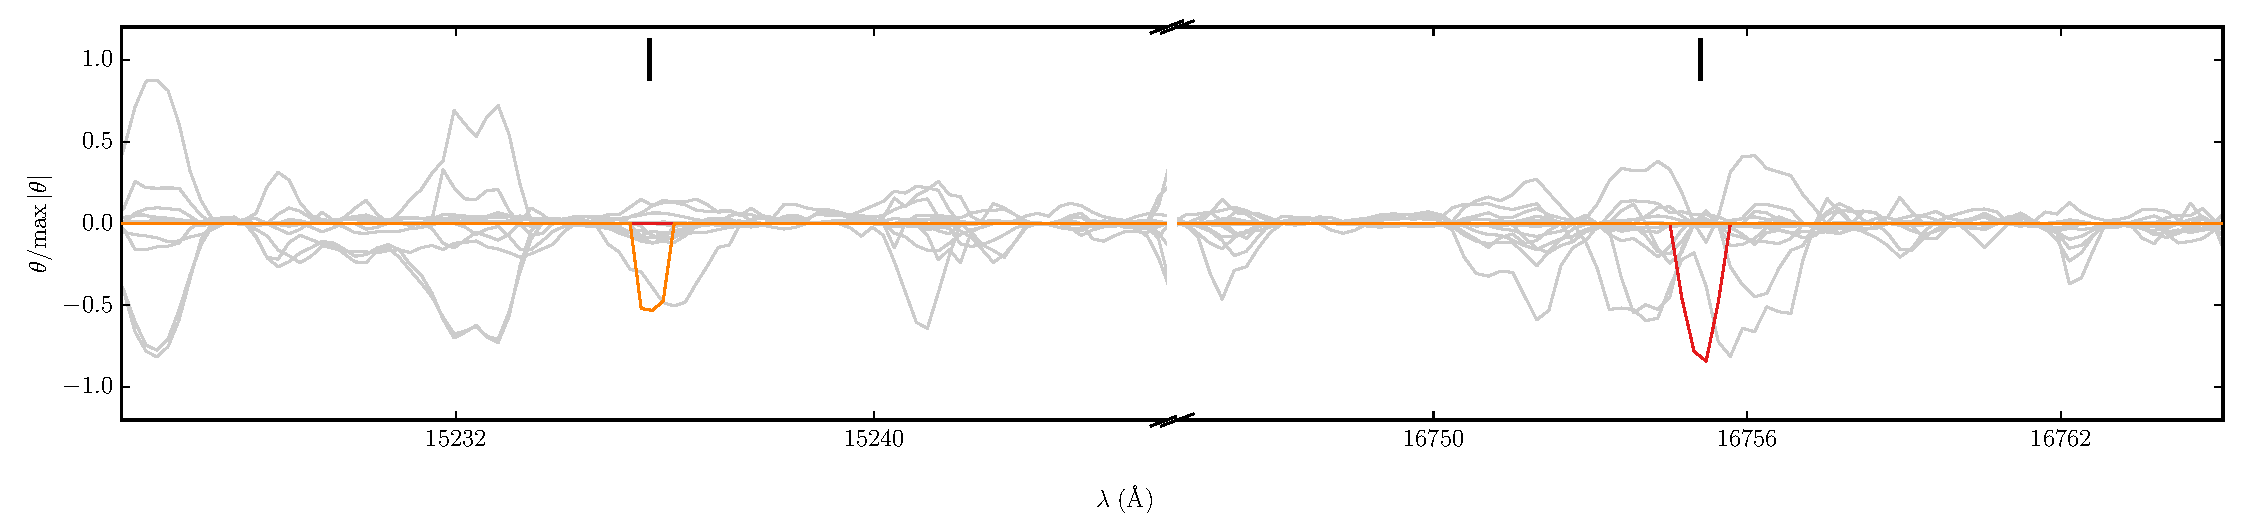
\includegraphics[width=\textwidth]{sparse-first-order-coefficients-zoom.pdf}
\caption{Zoom in of previous figure, showing the theta values for all elements. Al and S are highlighted and colored as per Figure \ref{fig:inferring-lines}.\label{fig:inferring-lines2}}
\end{figure}

\end{document}
